% $Header: /cvsroot/latex-beamer/latex-beamer/solutions/generic-talks/generic-ornate-15min-45min.en.tex,v 1.5 2007/01/28 20:48:23 tantau Exp $

\documentclass[xcolor=pdftex,dvipsnames,table,svgnames,x11names]{beamer}

% This file is a solution template for:

% - Giving a talk on some subject.
% - The talk is between 15min and 45min long.
% - Style is ornate.



% Copyright 2004 by Till Tantau <tantau@users.sourceforge.net>.
%
% In principle, this file can be redistributed and/or modified under
% the terms of the GNU Public License, version 2.
%
% However, this file is supposed to be a template to be modified
% for your own needs. For this reason, if you use this file as a
% template and not specifically distribute it as part of a another
% package/program, I grant the extra permission to freely copy and
% modify this file as you see fit and even to delete this copyright
% notice. 

\mode<handout>{
  \usepackage{pgfpages}
  \pgfpagesuselayout{4 on 1}[a4paper,border shrink=5mm]
}
\mode<presentation>{	
  \usetheme{Warsaw}
  \setbeamertemplate{caption}[numbered]
}
\usepackage{url}
\usepackage[english]{babel}
% or whatever
\usepackage{fancybox}
\usepackage[latin1]{inputenc}
% or whatever

\usepackage{times}
\usepackage[T1]{fontenc}
% Or whatever. Note that the encoding and the font should match. If T1
% does not look nice, try deleting the line with the fontenc.


\title % (optional, use only with long paper titles)
{Hard Errors}

\subtitle
{Mechanisms and Mitigation} % (optional)

\author % (optional, use only with lots of authors)
{Smruti R. Sarangi}
% - Use the \inst{?} command only if the authors have different
%   affiliation.

\institute[Universities of Somewhere and Elsewhere] % (optional, but mostly needed)
{
  Department of Computer Science\\
  Indian Institute of Technology \\
  New Delhi, India 
}
% - Use the \inst command only if there are several affiliations.
% - Keep it simple, no one is interested in your street address.
\date{}
\subject{Lectures}
% This is only inserted into the PDF information catalog. Can be left
% out. 

\renewcommand{\raggedright}{\leftskip=0pt \rightskip=0pt plus 0cm} 

% If you have a file called "university-logo-filename.xxx", where xxx
% is a graphic format that can be processed by latex or pdflatex,
% resp., then you can add a logo as follows:

% \pgfdeclareimage[height=0.5cm]{university-logo}{university-logo-filename}
% \logo{\pgfuseimage{university-logo}}



% Delete this, if you do not want the table of contents to pop up at
% the beginning of each subsection:
\AtBeginSubsection[]
{
  \begin{frame}<beamer>{Outline}
    \tableofcontents[currentsection,currentsubsection]
  \end{frame}
}


% If you wish to uncover everything in a step-wise fashion, uncomment
% the following command: 

%\beamerdefaultoverlayspecification{<+->}


\begin{document}

\begin{frame}
  \titlepage
\end{frame}

% This is the main Outline Section
\begin{frame}{Outline}
  \tableofcontents
  % You might wish to add the option [pausesections]
\end{frame}


% Since this a solution template for a generic talk, very little can
% be said about how it should be structured. However, the talk length
% of between 15min and 45min and the theme suggest that you stick to
% the following rules:  

% - Exactly two or three sections (other than the summary).
% - At *most* three subsections per section.
% - Talk about 30s to 2min per frame. So there should be between about
%   15 and 30 frames, all told.

\section{Introduction}

\begin{frame} {Motivation}
 \begin{example}
    Let us assume that we want to run a 1024 node server for a bank. The server needs to run 24x7. 
    Moreover, we have the following requirements for financial applications
      \begin{itemize}
       \item Preferably zero down time
       \item \alert{Absolutely no data corruption}
       \item Data security
       \item Maintainability, Serviceability
      \end{itemize}
 \end{example}

\begin{block} {}
  Let us focus on \underline{zero down time}, and \underline{no data corruption} in this talk.  
\end{block}

\end{frame}

\begin{frame}[shrink]{Motivation-II}
  \begin{block}{Zero Down Time}
    We would ideally want a computer for any kind of a critical application :banking, insurance, military, aerospace, 
    to be on most of the time. Failures can be catastrophic if computers start failing on planes and space crafts. 
    For critical applications like aerospace, we desire a failure rate as close to 0\% as possible. However, for 
    most financial applications, we are fine with 99.999\% (5 9s reliability). This translates to about 5 mins per year.
    If there are 1000 nodes on a server, then the failure rate per node needs to be pretty small.
  \end{block}
  \begin{block}{No Data Corruption}
    It is possible that because of computer faults, a bit can get inverted. This is a very serious failure mechanism
    in financial applications. Imagine 10,000Rs becoming 2 crore 10,000 Rs, or the reverse !!!
  \end{block}
\end{frame}

\begin{frame}[shrink=10]{Definition of Hard Errors}
We will discuss \emph{Hard Errors} in this chapter. 
\begin{definition}[Hard Error]
These errors are caused by defects in the silicon, or in the metalization, in the processor package.
They are permanent in nature.
\end{definition}
\pause
There are two kinds of hard errors

\begin{itemize}
 \item \textbf{Extrinsic}
    \begin{itemize}
      \item Contaminants on the silicon surface
      \item Open and short circuits
      \item Most of them are detected in the \textit{Burn-In} process
      \item They are like birth defects. Most of them are detected in the Burn-In process.
    \end{itemize}
\pause
 \item \textbf{Intrinsic}
    \begin{itemize}
    \item Caused by wear and tear
    \item These are age related defects that increase over time
    \end{itemize}
\end{itemize}
\end{frame}

\section{Different Types of Hard Errors}
\begin{frame}{Reliability Challenges}
Common failure modes

\begin{itemize}

 \item \textcolor{Navy}{Electomigration} 
    \begin{itemize}
    \item Over time the structure of a wire changes. Metal atoms tend to amass at one end 
    at one end of the wire. 
    \end{itemize}
\pause
 \item \textcolor{Navy}{Stress Migration }
    \begin{itemize}
    \item  Because of varying amounts of thermal expansion along a wire, electrons migrate to
	  different parts of the wire.
    \end{itemize}
\pause
 \item \textcolor{Navy}{Time Dependent Dielectric Breakdown}
    \begin{itemize}
      \item The gate dielectric in a transistor gradually breaks down over time. It ultimately becomes
      a short circuit.
    \end{itemize}
\pause
 \item \textcolor{Navy}{Thermal Cycling}
    \begin{itemize}
    \item The solder joints between the package and die interface experience constant changes in 
    temperature. This causes metal fatigue, and ultimate breakage.
    \end{itemize}
\end{itemize}
\end{frame}

\subsection{Failure Modes}
\begin{frame}{Electromigration}
 \begin{block}{}
Conducting electors in aluminum or copper interconnects transfer some of their momentum to surrounding
metal atoms. These metal atoms slowly drift along with the electrons. Over time, atoms from one end 
drift and accumulate at the other end. The depletion sites exhibit increased resistance. Finally, the
wire ceases to conduct.
\end{block}
\begin{displaymath}
 MTTF_{em} \propto (J - J_{crit})^{-n}e^{\frac{E_{aEM}}{kT}}
\end{displaymath}
\begin{itemize}
 \item $n$ and $E_{aEM}$ are constants that depend on the metal type. They are close to 1.
 \item $J$ is the current density. $J_{crit}$ is typically 2 orders of magnitude smaller than $J$. 
\end{itemize}

\end{frame}

\begin{frame}{Electromigration II}
 \begin{displaymath}
    J = \frac{CV_{dd}}{WH} * f * p 
\end{displaymath}
\begin{itemize}
 \item $C$: capacitance, $V_{dd}$: supply voltage, $W$: width
 \item $H$: height, $f$: frequency, $p$: switching probability
\end{itemize}
\begin{figure}[h]
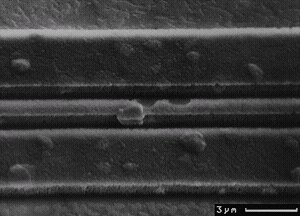
\includegraphics[width=1.5in]{electromigration}
\caption{\footnotesize Electromigration (courtesy: Philip Koopman, CMU) }
\end{figure}
\end{frame}


\begin{frame}{Stress Migration}

 \begin{block}{}
  This is a phenomenon similar to electromigration. Atoms migrate because of a variable amount of thermal
expansion. This thermomechanical stress gives wires and contacts irregular shapes. Much of the reasons
behind stress migration are not well understood.
  \end{block}

\begin{displaymath}
 MTTF_{sm} \propto |T_0 - T|^{-n}e^{\frac{E_{aSM}}{kT}} 
\end{displaymath}

\begin{itemize}
\item $T_0$: Temperature at which the metal was originally deposited (500K)
\item $T$: Operating temperature, $E_{aSM}$ and $n$ are material dependent constants
\item $E_{aSM}=2.5$ and $n=0.9$ for copper interconnects
\end{itemize}

\end{frame}

\begin{frame}{Time Dependent Dielectric Breakdown}
\begin{figure}[h]
 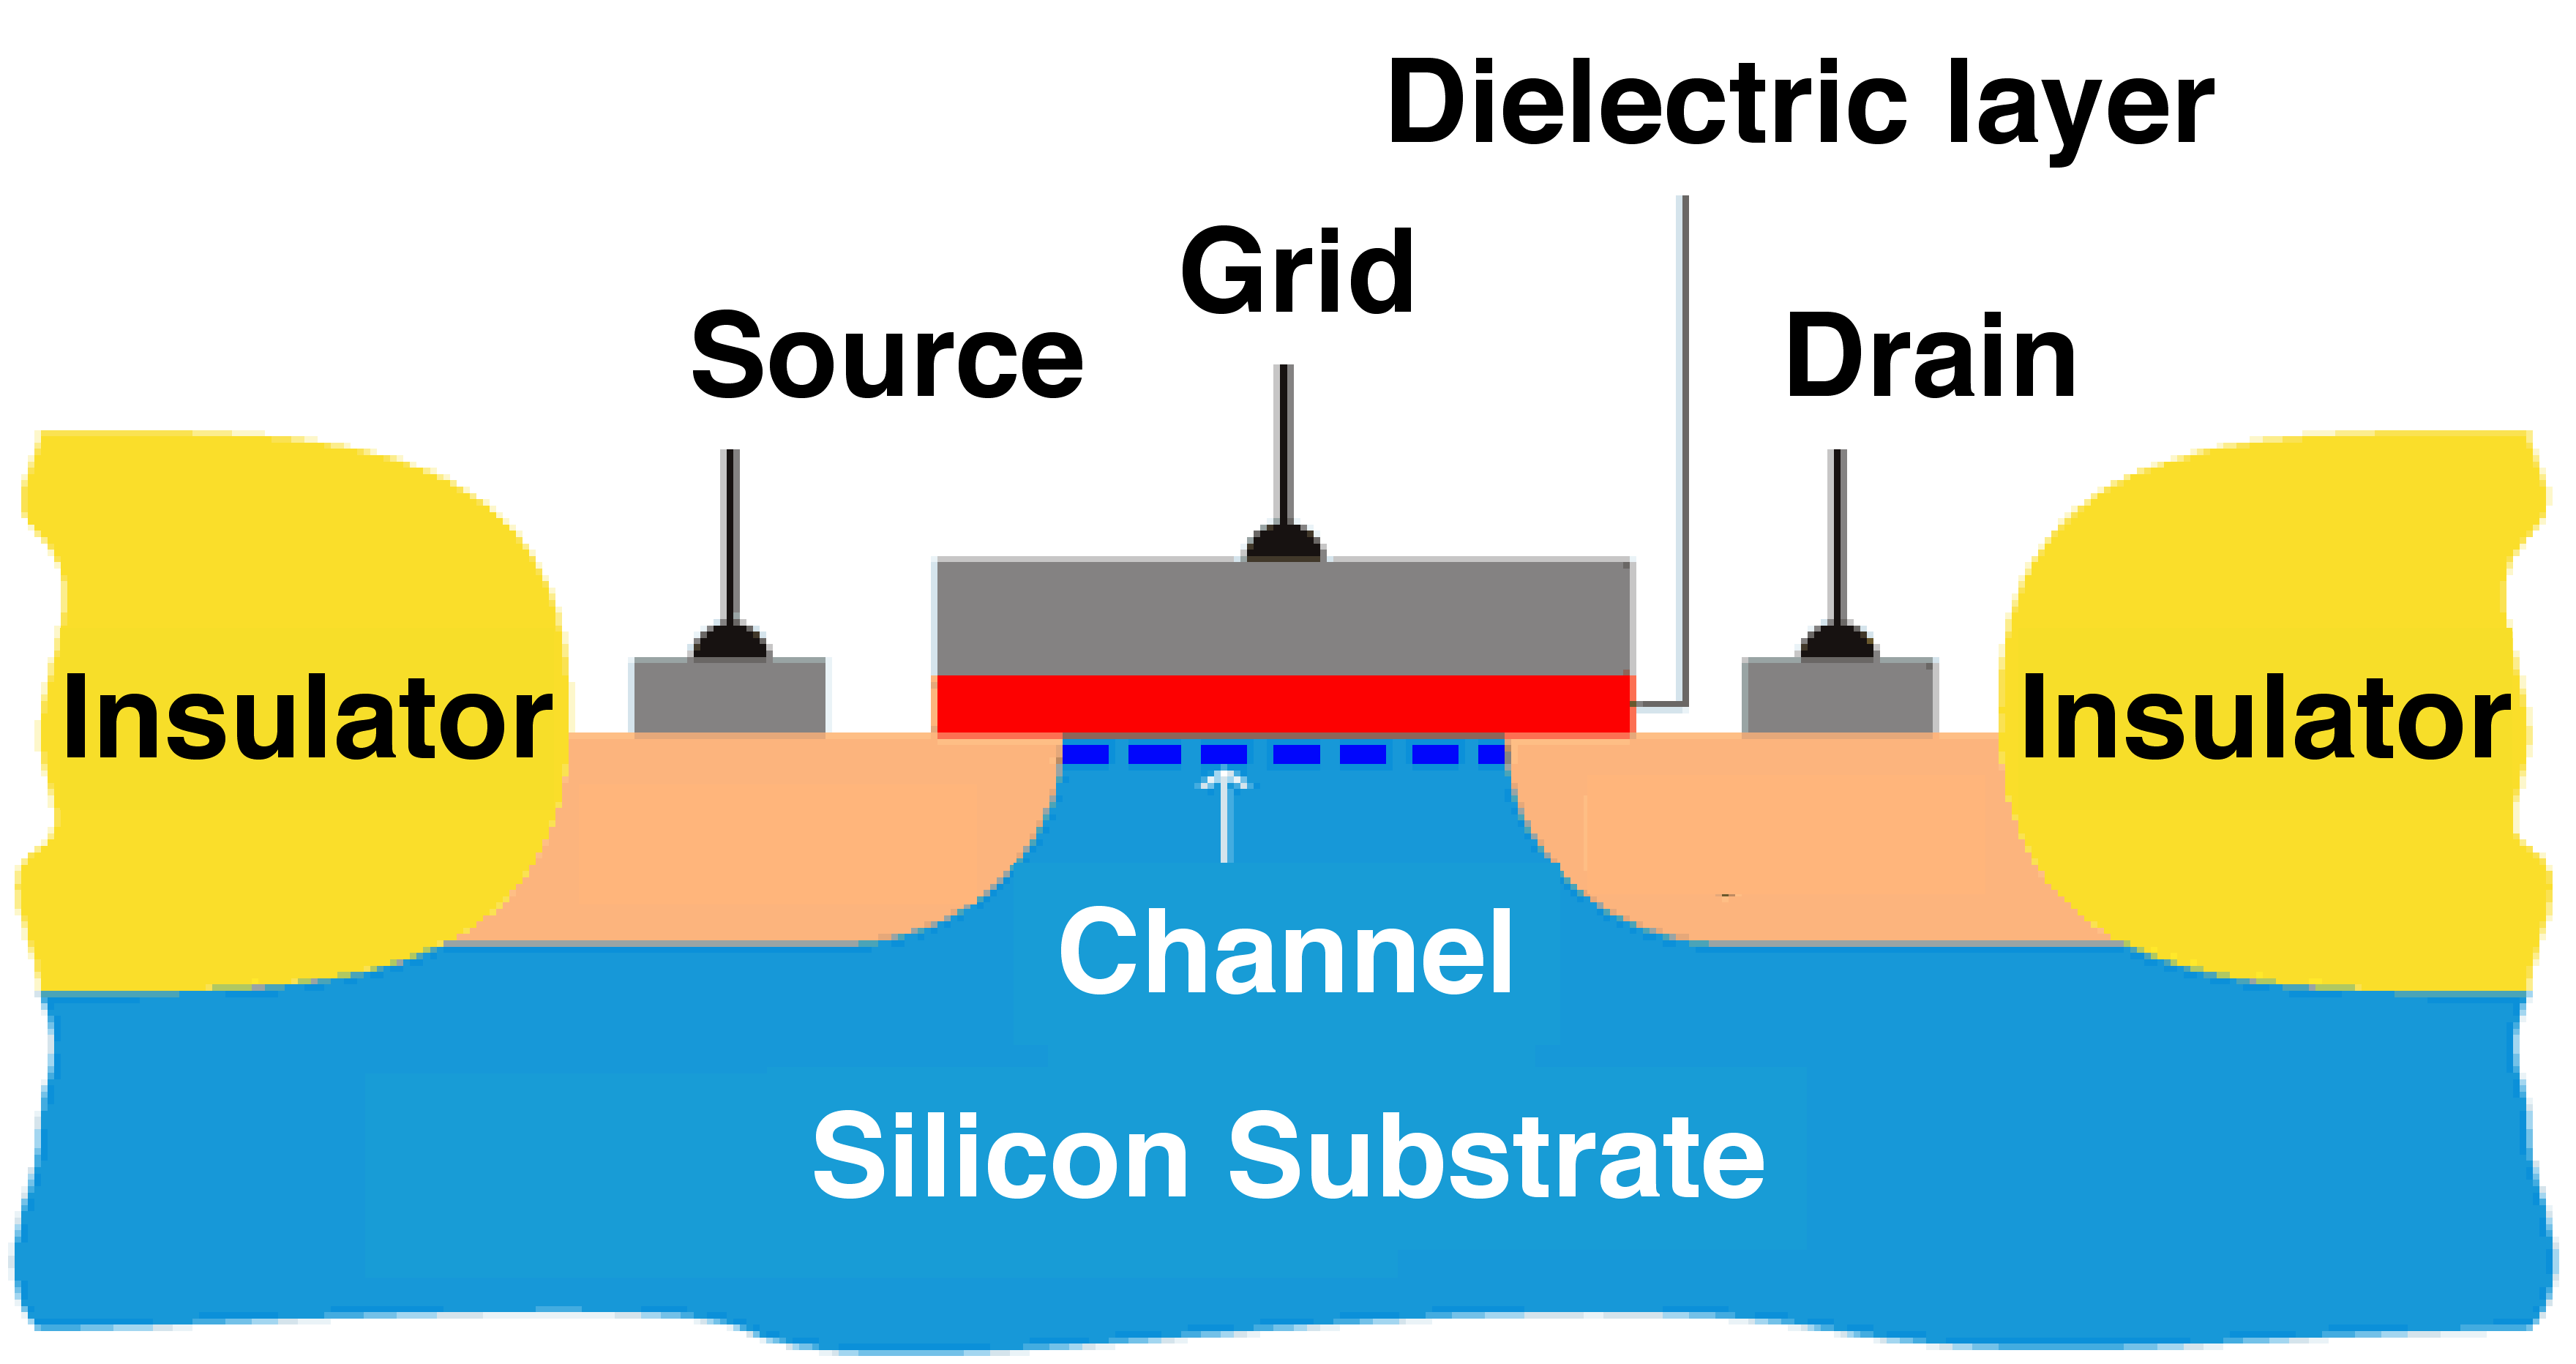
\includegraphics[width=4cm]{mos}
\caption{\footnotesize MOS Transistor (courtesy Gian-Marco Rignanese)}
\end{figure}

\begin{figure}[h]
 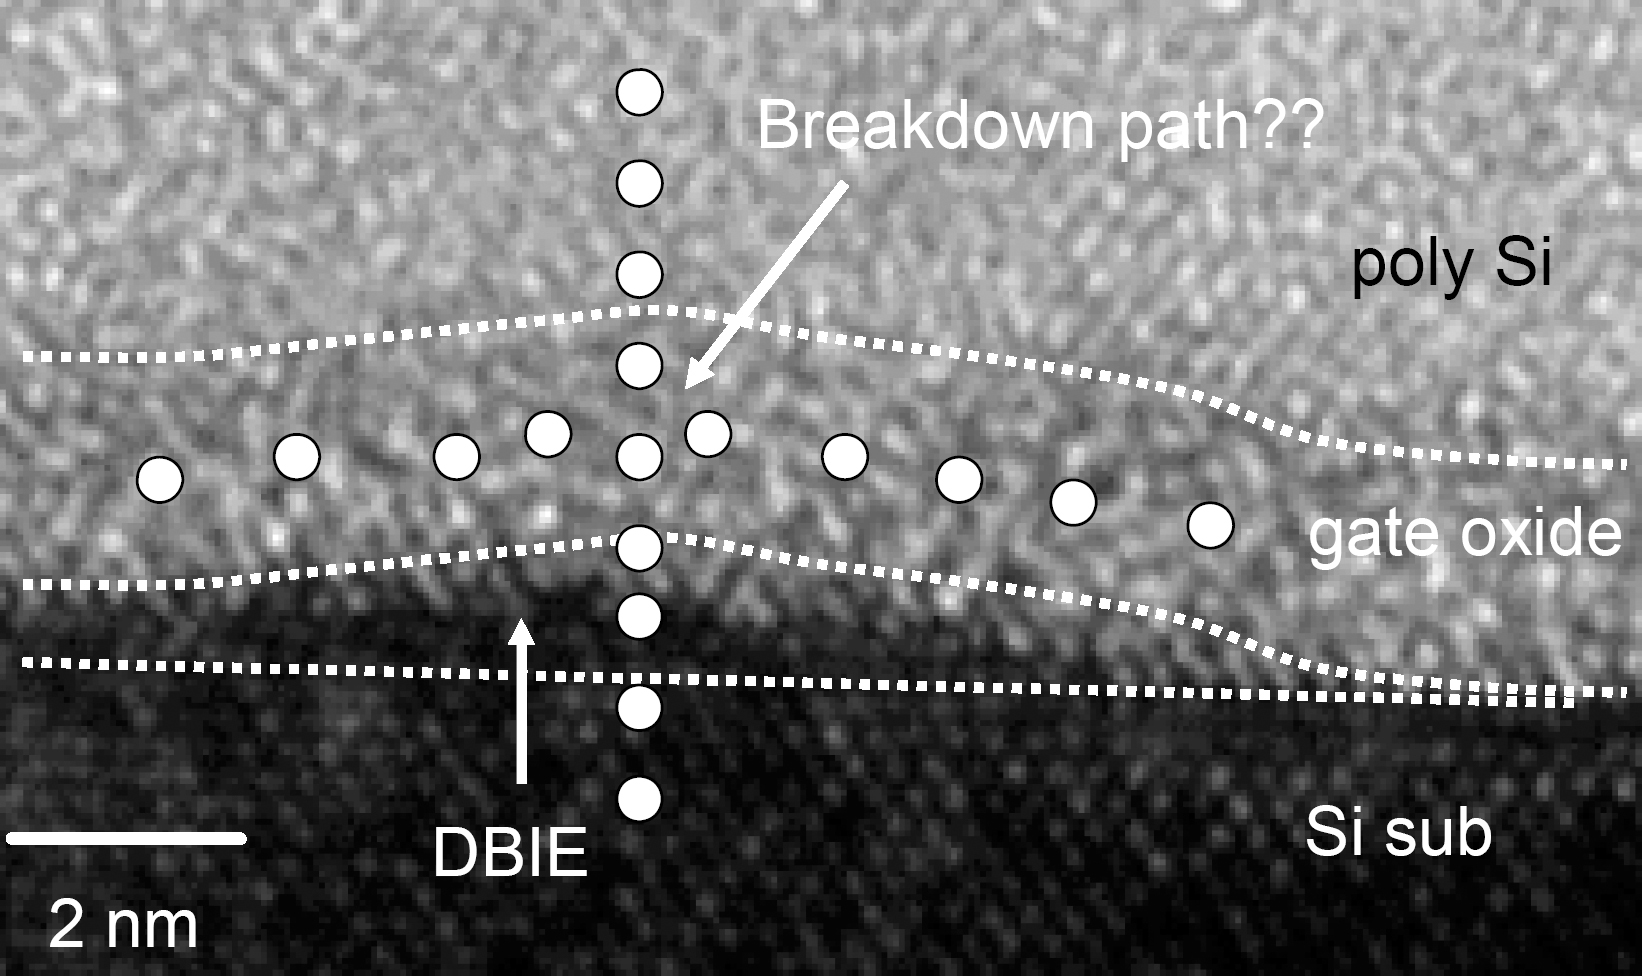
\includegraphics[width=4cm]{dielectric_breakdown}
\caption{\footnotesize Dielectric Breakdown (courtesy Kin-Leong Pey)}
\end{figure}
\end{frame}

\begin{frame} {Time Dependent Dielectric Breakdown - II}
\begin{block}{}
 The gate dielectric is typically very thin (about 2 nm). Over time it wears down and 
current passes through it. It forms a conducting path. It is hyper-exponentially
dependent on temperature.
\end{block}

\begin{displaymath}
 MTTF_{tddb} \propto \frac{1}{V}^{(a-bT)}e^{\frac{X+\frac{Y}{T} +ZT}{kT}}
\end{displaymath}

\end{frame}

\begin{frame}{Thermal Cycling - Metal Fatigue}
\begin{figure}[h]
 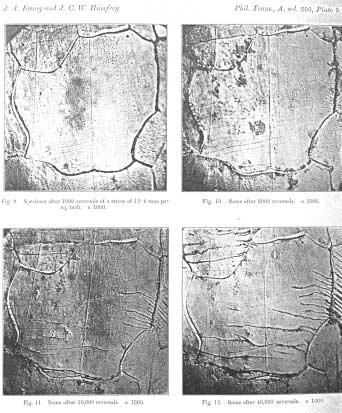
\includegraphics[width=4cm]{fatigue_cracks}
\caption{\footnotesize Metal Fatigue (wikipedia)}
\end{figure}
\end{frame}

\begin{frame}{Thermal Cycling-II}
\begin{itemize}
 \item Cycles of expansion and contraction give rise to metal fatigue especially at the I/O contacts.
 \item Over time, cracks begin to form
 \item There are two kinds of thermal cycles
      \begin{itemize}
	  \item Large cycles : Powering up/down the processor
	  \item Small cycles: Periods of activity/inactivity while executing a workload.
      \end{itemize}
\end{itemize}

\fbox{Coffin Manson Equation}
  \begin{block}{}
\begin{displaymath}
 MTTF_{tc} \propto \left ( \frac{1}{T - T_{ambient}} \right )^q 
\end{displaymath}
\end{block}
\begin{itemize}
 \item q = 2.35 in the reference.
\end{itemize}

\end{frame}

\subsection{Combining Failure Rates}
\begin{frame}{Sum of Failure Rates Model}
\begin{block}{Assumptions}
 \begin{itemize}
   \item The processor is a series failure system. One failure makes the entire processor fail.
  \item Every failure mechanism has an exponential distribution. 
 \end{itemize}
\end{block}
\begin{definition}{Failure Rate $h(t)$: }
 It is the conditional probability that a component will fail between $t$ and $(t + \delta t)$, given
the fact that it has survived till $t$. $h(t) = \lambda$, means that the application has a constant failure
rate.
\end{definition}
\begin{example}
 The exponential distribution $f(x) = \lambda e^{-\lambda x}$, has a constant failure rate, $\lambda$. 
\end{example}
\end{frame}

\begin{frame}{Sum of Failure Rates Model - II}
 \begin{definition}{FIT: }
  Failure-in-time. The number of failures in a billion hours.
 \end{definition}

\begin{displaymath}
 MTTF_p = \frac{1}{\lambda_p} = \frac{10^9}{FIT}=\frac{1}{\sum_i\sum_j \lambda_{ij}}
\end{displaymath}

\begin{itemize}
 \item $\lambda_{ij}$ is the failure rate of $i_{th}$ structure due to the $j_{th}$ failure mechanism.
\end{itemize}
\end{frame}

\begin{frame}[shrink]{Mathematical Trivia}
 \begin{Theorem}
  The failure rate for the exponential distribution is $\lambda$. 
 \end{Theorem}
\begin{Proof}
 Let the time of failure be $t_f$. Let the failure rate be $h(t)$. The exponential
equation for the pdf of the failure is $f(t) = \lambda e^{-\lambda t}$. We have:
\begin{equation}
\begin{split}
  h(t) & = P(t \le t_f \le t + \delta t  | t_f < t)  \\
       & = \frac{P( (t \le t_f \le t + \delta t) \wedge (t_f < t) )}{P(t_f < t) } \\
       & = \frac{f(t)}{1- \int_0^t f(x)} \\
       & = \frac{\lambda e^{-\lambda t}}{e^{-\lambda t}} \\
       & = \lambda \\
 \end{split}
\end{equation}

\end{Proof}
\end{frame}


\begin{frame}[shrink]{Mathematical Trivia - II}
 \begin{Theorem}
  The MTTF for the exponential distribution is $\frac{1}{\lambda}$. 
 \end{Theorem}
\begin{Proof}
 The exponential
equation for the pdf of the failure is $f(t) = \lambda e^{-\lambda t}$. We have:
\begin{equation}
\begin{split}
  MTTF &= \int_0^{\infty} t f(t) dt \\
    &= \int_0^{\infty} t \lambda e^{-\lambda t} dt \\
    &= \frac{1}{\lambda} \int_0^{\infty} x e^{-x} dx \quad (x=\lambda t) \\
    &= \frac{1}{\lambda} \left ( (-x e^{-x})  \mid_0^{\infty} +  \int_0^{\infty} e^{-x} dx \right ) \\
    &= \frac{1}{\lambda} \\
 \end{split}
\end{equation}
\end{Proof}
\end{frame}

\begin{frame}[shrink=10]{RAMP Model}
\begin{block}{Assumptions}
 \begin{itemize}
    \item Processors are designed to have an MTTF of 30 years.
    \item The FIT value is therefore 4000. 
    \item Worst case operating conditions will lead to a failure rate of 30 years.
    \item The total failure rate is distributed evenly across the four failure modes.
 \end{itemize}
\end{block}
Let us now try to find the constants in the equations.
\begin{itemize}
 \item There are four parameters considered : $T$, $V$, $f$, and $p$(activity factor)
 \item Let there values for the worst case be : $T_{qual}$, $V_{qual}$, $f_{qual}$, and $p_{qual}$.
 \item $V_{qual}$ is the highest supply voltage (about 1.2 V), $f_{qual}$ is the highest frequency
 \item $p_{qual}$ is 1. $T_{qual}$ is dependent on the manufacturing specs. Typically 393K (120 $^\circ$C).
\end{itemize}
\end{frame}

\begin{frame}{Ramp Model Contd... }
 \begin{itemize}
  \item $T_{qual}$ is typically provided by the manufacturer.
  \item Most references assume a value of 120 $^\circ$C.
  \item The RAMP model computes the values of the proportionality constants for the four failure modes
  \item The RAMP paper evaluates the hard error FIT rates for different configurations.
 \end{itemize}
\end{frame}

\subsection{RAMP-II}
\begin{frame}[shrink=5]{Normal Distribution}
 \begin{block}{Central Limit Theorem}
  Let ($x_1$, \ldots, $x_n$) be a sequence of numbers that are identically and independently distributed(i.i.d). The sum of the
sequence for large values of  $n$, is normally distributed.
 \end{block}
\textcolor{Blue3}{\underline{Normal distribution:}}
\begin{equation*}
 f(x) = \frac{1}{\sigma \sqrt{2\pi}} e^{-\frac{(x-\mu)^2}{2\sigma^2}}
\end{equation*}

\begin{itemize}
  \item $\mu$ is the mean, $\sigma$ is its variance
 \item The normal distribution is thus a very fundamental distribution. 
  \item Most natural phenomena are modeled by this distribution, or by variants of it.
\end{itemize}

\end{frame}

\begin{frame}[shrink=3]{Log-Normal Distribution}
\begin{itemize}
  \item The exponential distribution has a constant failure rate. 
      \begin{itemize}
       \item Most failure rates increase over time
	\item This is not an \textcolor{SlateBlue4}{accurate} assumption
      \end{itemize}
  \item Such kind of failures are typically model by \textcolor{Blue3}{log-normal} distributions
    \begin{itemize}
      \item $x$ has a log-normal distribution, if $ln(x)$ has a normal distribution
    \end{itemize}
\end{itemize}

\textcolor{Blue3}{\underline{Log-Normal distribution:}}
\begin{equation*}
 f(x) = \frac{1}{x\sigma \sqrt{2 \pi}} e ^ {-\frac{(ln(x) - \mu)^2}{2\sigma^2}} \quad, x>0
\end{equation*}
\end{frame}



\begin{frame}{Food for Thought}
\begin{center}
\vspace{-9mm}
 \begin{figure}[h]
    
\includegraphics[width=1.3in]{burger}
 \end{figure}
\vspace{-7mm}
\end{center}
  \begin{block}{Question}
    Let us consider a failure process, in which the amount of degradation between the time instants, $t_n$ and $t_{n-1}$
    is proportional to the degradation at $t_{n-1}$. If the degradation at $t_n$ is $x_n$, we have: $x_n - x_{n-1} = \alpha_n x_{n-1}$. 	
    Let us further assume that $\alpha_n$ has an i.i.d distribution. Prove that $x_n$ has a log-normal distribution.
  \end{block}
\end{frame}

\begin{frame}{NBTI (Not in course ...)}
\begin{itemize}
 \item RAMP-II adds a fifth failure mode called \textcolor{Blue3}{NBTI}
    \begin{itemize}
      \item NBTI : Negative bias temperature instability
    \end{itemize}
\end{itemize}
\begin{definition}{NBTI: }
 When the p-FET gate is biased negative w.r.t to the drain and source, then positive charge tends to accumulate on the
	  gate oxide. This accumulation causes the threshold voltage of the transistor to increase, ultimately leading to its
	  failure.
\end{definition}
\begin{equation*}
 MTTF \propto \left [ \left (ln \left (\frac{A}{1 + 2e^{\frac{B}{kT}}} \right ) -  ln \left (
	  \frac{A}{1 + 2e^{\frac{B}{kT}}} -C \right ) \right) * \frac{T}{e^{-\frac{D}{kT}}}\right ]^{\frac{1}{\beta}}
\end{equation*}
\end{frame}

\section{Prevention and Recovery}

\begin{frame}{Duplication}
 \begin{itemize}
  \item Duplication : Maintain multiple copies of a functional unit 
    \begin{itemize}
      \item Example : Two adders, or two versions of the fetch unit
      \item Keep one unit permanently powered off
      \item When the first unit fails, switch to the second one
      \item \textcolor{red}{Negative Point: } We are increasing the area of the chip in the process
    \end{itemize}
 \end{itemize}
\begin{center}
\begin{figure}[h]
 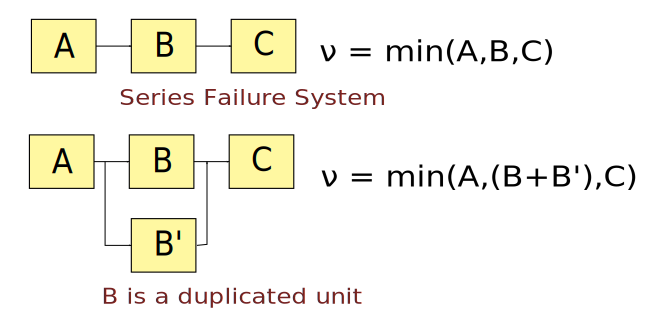
\includegraphics[width=3in]{map1}
\end{figure}
\end{center}

\end{frame}

\begin{frame} {Graceful Degradation}
\begin{itemize}
  \item Degradation : Gradually reduce the functionality of a unit 
    \begin{itemize}
      \item Example : We can gradually decrease the size of buffers like the branch predictor. This will decrease
	    performance but not correctness.
      \item The instruction queue can be segmented. We can gradually decrease the number of segments.
      \item \textcolor{red}{Positive Point: } Very little area penalty
    \end{itemize}
 \end{itemize}

\begin{center}
\begin{figure}[h]
 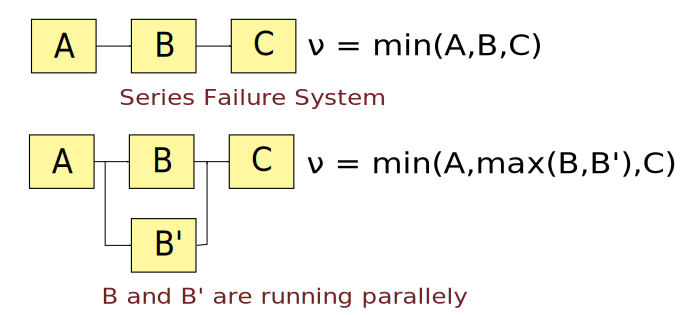
\includegraphics[width=3in]{map2}
\end{figure}
\end{center}

\end{frame}

\begin{frame}{Food for Thought}
\begin{center}
  \begin{figure}[h]
    
\includegraphics[width=1.3in]{burger}
 \end{figure}
 \end{center}
\vspace{-6mm}
 \begin{theorem}
  The distribution of the minimum of $n$ exponential random variables with rates, $\lambda_1, \ldots, \lambda_n$, is 
another exponential variable with rate, $(\lambda_1 + \ldots + \lambda_n)$. 
 \end{theorem}

\end{frame}

\begin{frame}[shrink=5] {Handling Faults in Memories}
 \begin{center}
  \begin{figure}[h]
   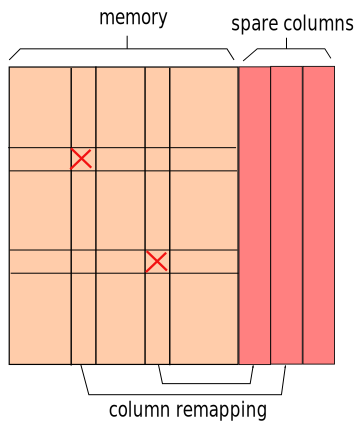
\includegraphics[width=1.65in]{memory}
  \caption{\footnotesize Remapping columns for a memory bank}
  \end{figure}
 \end{center}
\vspace{-7mm}
\begin{itemize}
 \item Perform a BIST (Built-in self test) to find faulty memory cells
  \item Change the decoder logic to map the columns with faulty cells to spare columns
  \item Can be done right after manufacturing, or can be done online
\end{itemize}

\end{frame}

% Bibliography
\bibliographystyle{plain}
\small
\begin{thebibliography}{10}
 \bibitem{lifetime}
The Case for Lifetime Reliability-Aware Microprocessors, Jayanth Srinivasan, 
Sarita V. Adve, Pradip Bose, and Jude A. Rivers, Proceedings of 31st International 
Symposium on Computer Architecture (ISCA '04) June 2004.\\
\url{http://rsim.cs.illinois.edu/~srinivsn/Pubs/isca04.pdf}

\bibitem{lifetimeii}
Jayanth Srinivasan, Sarita V. Adve, Pradip Bose, Jude A. Rivers: Exploiting Structural 
Duplication for Lifetime Reliability Enhancement. ISCA 2005: 520-531\\
\url{http://rsim.cs.illinois.edu/~srinivsn/Pubs/isca05.pdf}

\end{thebibliography}

\end{document}